\section{Meta-modelling}

\noindent
\todo{What is meta-modelling? Can get this from honours thesis...?}

To understand the methodology on how we captured our dataset, we must first introduce the three key notions behind \gls{mde}: technical spaces, models and systems. A system is a concrete ``group or set of related or associated elements perceived or thought of as a unity or complex whole'' \citep{OEDDefintion:System}. Technical spaces were introduced by \citet{Bezivin:2002} as a model management framework based on algebraic structures (e.g., trees, (hyper)graphs, and categories). Technical spaces are usually based on a three-tier conjecture: meta-meta-models, meta-models and models. Whereas a model is an abstract representation of  a concrete system of specific purpose, a \textit{meta}-model, in contrast, describes the way to describe those models. A \textit{meta-meta}-model can be used to describe the representation structure of our meta-models and defines a type system \cite{Cardelli:1985ee} that supports all underlying layers \citep{Bezivin:2006gw}. \cref{fig:literature-review:metamodelling:metamodel} captures these concepts in further detail.

\begin{figure}[h]
  \centering
  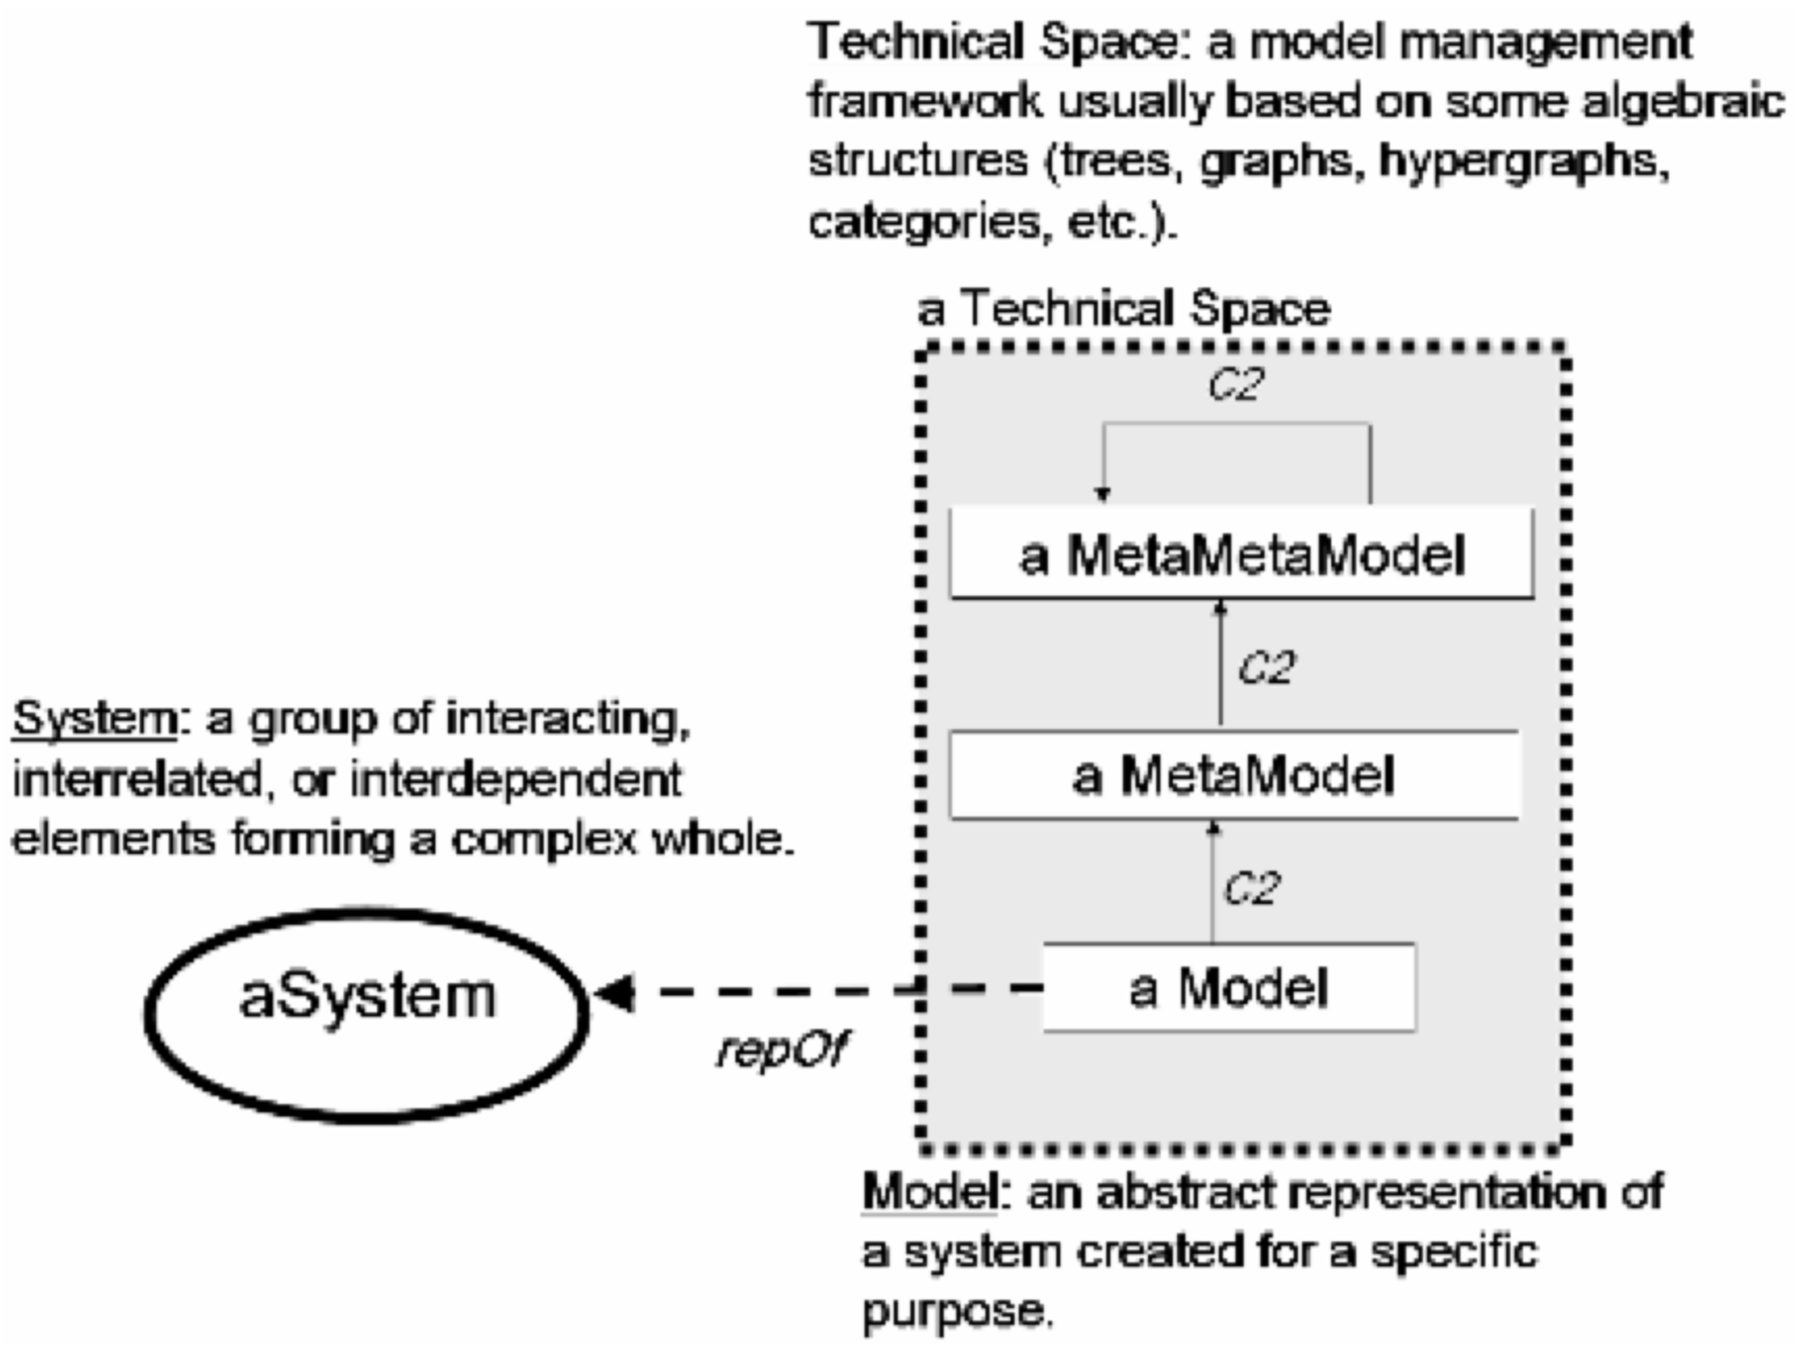
\includegraphics[width=0.6\textwidth]{bezivin2006_metamodel}
  \caption[An overview of systems, models and technical spaces]{Systems, models and technical spaces. (From \citep{Bezivin:2006gw}.)}
  \label{fig:literature-review:metamodelling:metamodel}
\end{figure}

\noindent
\todo{How does this differ in AI context?}